%% !TEX root = manual.tex

\section{Abstract Machine Models}
\label{sec:amm}

The preferred mode for usage of \sstmacro will be through specifying parameters for well-defined abstract machine models.
This represents an intermediate-level mode that should cover the vast majority of use cases.
The highly configurable, detailed parameter files will remain valid but will represent advanced usage mode for corner cases.
The primary advantage of the abstract machine models is a uniform set of parameters regardless of the underlying congestion model or accuracy level (Pisces or LogGOPSim).
Each input file requires the usual set of software parameters given in \ref{sec:parameters}.
For hardware parameters, two initial parameters are required and one is optional.

\begin{ViFile}
congestion_model = pisces
amm_model = amm1
accuracy_parameter = 1024
\end{ViFile} 

Here we indicate the congestion model to be used (the packet-flow) and the overall machine model (abstract machine model \#1).
Currently valid values for the congestion model are \inlinefile{pisces} (most accurate, slowest) and \inlinefile{simple} (least accurate, fastest),
but more congestion models should be supported in future versions.
Currently valid values for the abstract machine model are \inlinefile{amm1}, \inlinefile{amm2}, \inlinefile{amm3}, see details below. 
Another model, \inlinefile{amm4}, that adds extra detail to the NIC is pending and should be available soon.
The details of individual abstract machine models are given in the following sections.
The optional accuracy parameter is less well-defined and the exact meaning varies considerably between congestion models.
In general, the accuracy parameter represents how coarse-grained the simulation is in bytes.
It basically corresponds to a packet-size. How many bytes are modeled moving through the machine separately at a time?
If the parameter is set to 8 bytes, e.g., that basically means we are doing flit-level modeling.
If the parameter is set to 8192 bytes, e.g. that means we are doing very coarse-grained modeling which only really affects large messages.
If the parameter is set to 100-1000 bytes, e.g., that means we are doing more fine-grained modeling on real packet sizes, but we are ignoring flit-level details.

\subsection{Common Parameters}
\label{subsec:commonParams}
The following parameters define the CPU and compute power of the node (independent of memory subsystem).
They are universal and are valid for all abstract machine models. 

\begin{ViFile}
node {
 model = simple
 frequency = 2.1ghz
 ncores = 24
 nsockets = 4
}
\end{ViFile}
or using the deprecated parameters:

\begin{ViFile}
node_name = simple
node_frequency = 2.1ghz
node_ccores = 24
node_sockets = 4
\end{ViFile}

\subsection{AMM1}
\label{subsec:ammOne}

\begin{figure}[h!]
\begin{center}
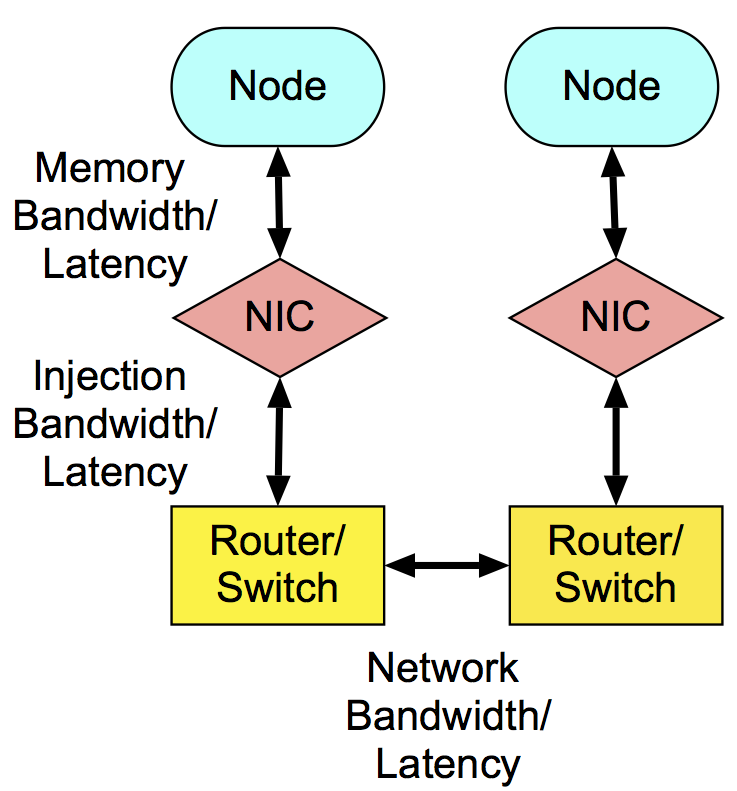
\includegraphics[width=0.4\textwidth]{figures/amm/AMM1.png}
\end{center}
\caption{AMM1: Used when focusing on network traffic only}
\label{fig:amm1}
\end{figure}

This is simplest abstract machine model and incorporates three basic components (i.e. congestion points).
Each node has a memory subsystem and NIC (injection/ejection).
Once packets are injected, they traverse a series of network switches.
The memory, injection, and network are all defined by a bandwidth/latency parameter pair.

\begin{ViFile}
network_link_bandwidth = 6GB/s
network_hop_latency = 100ns
injection_bandwidth = 10GB/s
injection_latency = 1us
memory_bandwidth = 10GB/s
memory_latency = 15ns
\end{ViFile}
These are special parameters used by the AMM configurations.
They can be by-passed by directly using fully namespaced parameters:

\begin{ViFile}
switch {
 link {
   bandwidth = 6GB/s
   latency = 100ns
 }
 ejection {
  latency = 100ns
  bandwidth = 10GB/s
 }
}
nic {
 injection {
  latency = 1us
  bandwidth = 10GB/s
 }
}
memory {
 bandwidth = 10GB/s
 latency = 15ns
}
\end{ViFile}

NOTE: there is no parameter \inlinefile{network_latency}.
The parameter is \inlinefile{network_hop_latency}.
This is the latency required for a single packet to traverse one switch and hop to the next one in the network.
Thus, even in the most basic of network models, there is a still a notion of topology that affects the number of hops and therefore the latency.
To compute the total network network latency as one would observe in an MPI ping-ping benchmark, one would compute
\[
lat = n_{hops} * lat_{hop} + 2*lat_{inj}
\]
using the hop latency and the injection latency.

This abstract machine model is a good place to start for getting a ``lay of the land'' for simulations - and the simplest to configure.
However, it has a few deficiencies that can cause problems when there is serious memory or network congestion.
More details (and their fixes) are given in the next abstract machine models. 	

\subsection{AMM2}
\label{subsec:amm2}

\begin{figure}
\begin{center}
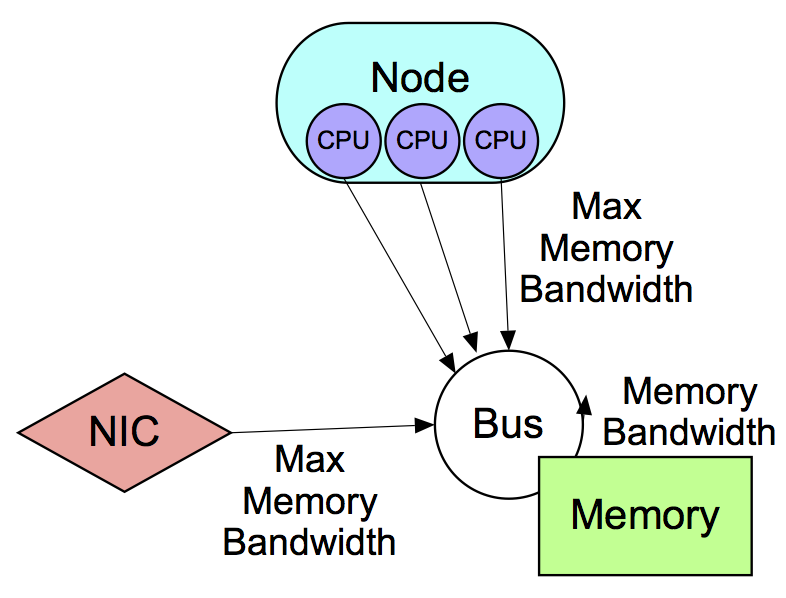
\includegraphics[width=0.4\textwidth]{figures/amm/amm2_membus.png}
\end{center}
\caption{AMM2: Adds extra memory model details to AMM1}
\label{fig:amm2}
\end{figure}

A major deficiency of AMM1 is that it grants exclusive access to memory resources.
Two CPUs or the NIC cannot be using the memory subsystem in parallel.
This is particularly problematic for large memory transfers (1 MB or greater).
The memory system might be blocked for approx 1 ms,
creating unphysical delays while other resources wait for access.
A more realistic model allows multiple resources to access the memory,
albeit with reduced bandwidth when congestion is observed.
In many cases, multiple memory links or management units are connect to a shared bus.
The bus determines to the total, aggregate memory bandwidth.
However, the individual links determine the maximum observed bandwidth by any single component.
AMM2 has all the same parameters as AMM1, but now allows an additional parameter for memory.
These are special parameters used by the AMM configurations.
They can be by-passed by directly using fully namespaced parameters (not shown).

\begin{ViFile}
max_memory_bandwidth = 5GB/s
memory_bandwidth = 10GB/s
memory_latency = 15ns
\end{ViFile}
The new parameter \inlinefile{max_memory_bandwidth} now defines the maximum bandwidth any single component is allowed.
Thus, even if the CPU is doing something memory intensive, 5 GB/s is still available to the NIC for network transfers.
We remark here that the memory parameters might be named something slightly more descriptive.
However, as a rule, we want the AMM1 parameters to be a proper subset of the AMM2 parameters.
Thus parameter names should not change - only new parameters should be added.

\subsection{AMM3}
\label{subsec:ammThree}

\begin{figure}
\begin{center}
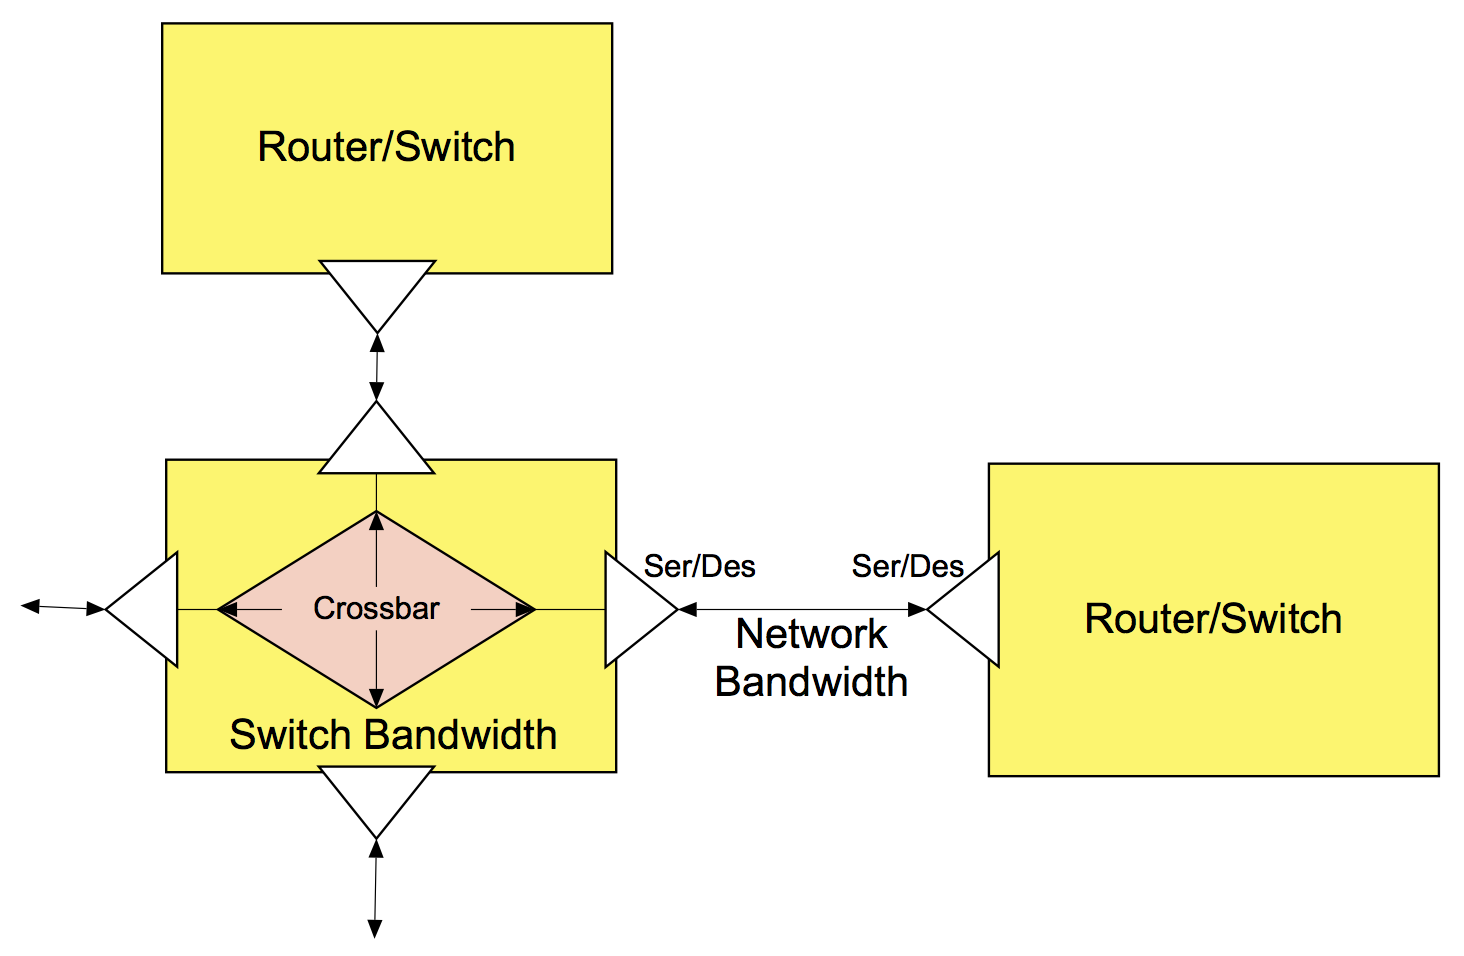
\includegraphics[width=0.5\textwidth]{figures/amm/amm3_switch.png}
\end{center}
\caption{AMM3: Adds extra router (switch) details to AMM2}
\label{fig:amm3}
\end{figure}

A major deficiency of AMM2 is its inability to distinguish between the network link bandwidth (associated with the outport port serializer/deserializer) and the switch bandwidth (associated with the crossbar that arbitrates packets).  
Only packets traveling the same path cause congestion on the network links in AMM1 and AMM2.
However, packets ``intersecting'' at a switch - even if following separate paths - can cause congestion through sharing the switching fabric.
AMM3 generalize the network parameters by adding a switch bandwidth.
We note again here that AMM3 has all the same parameters as AMM2, plus the additional switch bandwidth parameter.
Thus, higher-numbered abstract machine models always add more detail.
These are special parameters used by the AMM configurations.
They can be by-passed by directly using fully namespaced parameters (not shown) for more detailed configurations.

\begin{ViFile}
network_switch_bandwidth = 12GB/s
network_bandwidth = 6GB/s
network_hop_latency = 100ns
\end{ViFile}
